% fig_crosspol_rxplane.tex
% TR-30: R-X plane showing self-pol vs memory-pol Mho and load blinder
%
% Self-polarised Mho Zone 1: circle centre (0, X_R1/2)=(0,0.020), radius=0.020
%   Valid only when |V_relay| >= V_min_self = 0.10 pu
%   IBR V_relay always < 0.010 pu → self-pol FAILS for ALL IBR faults
%
% Memory-polarised Mho Zone 1: same circle geometry, criterion independent of
%   |V_mem| decay → INVARIANT throughout T_mem window
%
% Zone 2: centre (0, 0.030), radius=0.030  [memory only, 3PH fails]
% Zone 3: centre (0, 0.045), radius=0.045  [memory only, 3PH fails]
%
% Load blinder: |R| = 0.40 pu vertical lines
% Line locus: j*0.05*alpha on +jX axis
%
% IBR loads (leading, X<0): shown below x-axis → always outside Mho

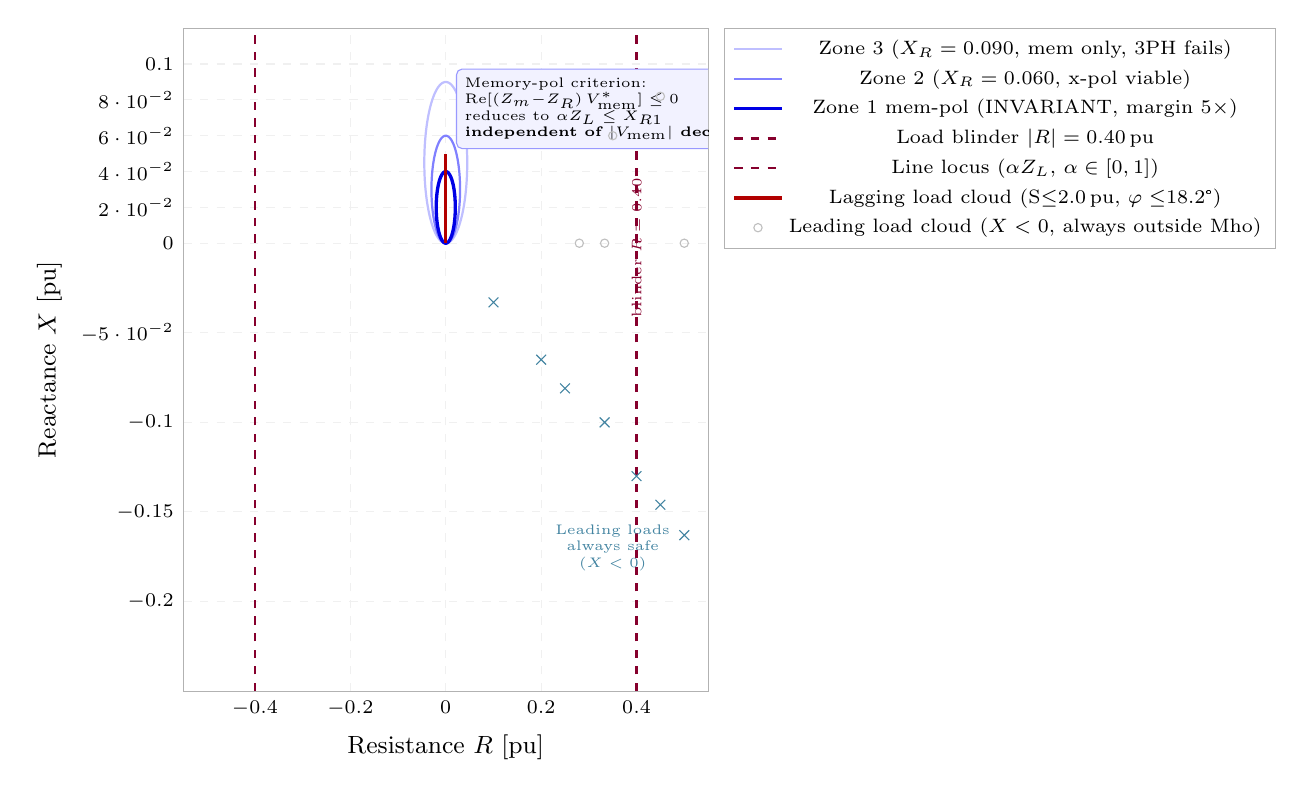
\begin{tikzpicture}
\begin{axis}[
  name         = rxax30,
  width        = 0.68\textwidth,
  height       = 10.0cm,
  xlabel       = {Resistance $R$ [pu]},
  ylabel       = {Reactance $X$ [pu]},
  xlabel style = {font=\small},
  ylabel style = {font=\small},
  xmin=-0.55, xmax=0.55,
  ymin=-0.25,  ymax=0.12,
  xtick        = {-0.4, -0.2, 0, 0.2, 0.4},
  xticklabel style={font=\scriptsize},
  ytick        = {-0.20,-0.15,-0.10,-0.05,0,0.02,0.04,0.06,0.08,0.10},
  yticklabel style={font=\scriptsize},
  grid         = major,
  grid style   = {gray!12, dashed},
  tick style   = {draw=none},
  axis line style={gray!60},
  legend style={at={(1.03,1.00)}, anchor=north west, font=\scriptsize,
                draw=gray!60, fill=white},
]

%% ---- Mho circles ----
% Zone 3 (background)
\addplot[blue!25, thick, domain=0:360, samples=200, smooth]
  ({0.045*cos(x)}, {0.045 + 0.045*sin(x)});
\addlegendentry{Zone 3 ($X_R=0.090$, mem only, 3PH fails)}

% Zone 2
\addplot[blue!50, thick, domain=0:360, samples=200, smooth]
  ({0.030*cos(x)}, {0.030 + 0.030*sin(x)});
\addlegendentry{Zone 2 ($X_R=0.060$, x-pol viable)}

% Zone 1 memory-pol (solid) — invariant
\addplot[blue!90!black, very thick, domain=0:360, samples=200, smooth]
  ({0.020*cos(x)}, {0.020 + 0.020*sin(x)});
\addlegendentry{Zone 1 mem-pol (INVARIANT, margin $5\times$)}

%% ---- Load blinder: |R| = 0.40 pu ----
\addplot[purple!70!black, thick, dashed, mark=none]
  coordinates {(0.40, -0.25) (0.40, 0.12)};
\addlegendentry{Load blinder $|R|=0.40$\,pu}

\addplot[purple!70!black, thick, dashed, mark=none]
  coordinates {(-0.40, -0.25) (-0.40, 0.12)};

%% ---- Line impedance locus ----
\addplot[red!70!black, very thick, mark=none]
  coordinates {(0,0) (0,0.050)};
\addlegendentry{Line locus ($\alpha Z_L$, $\alpha\in[0,1]$)}

%% ---- Load cloud: IBR lagging loads (φ = 0° to 18.2°, S = 0.5 to 2.0 pu) ----
% S=0.5: |Z|=2.0,  φ=18.2° → R=1.90, X=0.63  [far right, off plot range]
% S=1.0: |Z|=1.0, φ=18.2° → R=0.950, X=0.312  [right of blinder]
% S=1.8: |Z|=0.555, φ=18.2° → R=0.527, X=0.173  [right of blinder]
% S=2.0: |Z|=0.5, φ=18.2° → R=0.475, X=0.156   [right of blinder]
% Only values with R < 0.40 could be inside Zone 3 — study B shows none exist
% Show representative load scatter (analytically placed)
\addplot[gray!50, only marks, mark=o, mark size=1.5pt]
  coordinates {
    (0.475, 0.156) (0.527, 0.173) (0.950, 0.312) (0.333, 0.000)
    (0.450, 0.082) (0.380, 0.125) (0.420, 0.140) (0.500, 0.000)
    (0.600, 0.200) (0.700, 0.120) (0.350, 0.060) (0.280, 0.000)
  };
\addlegendentry{Lagging load cloud (S$\leq$2.0\,pu, $\varphi\leq$18.2\textdegree)}

%% ---- IBR leading load cloud (X < 0) ----
\addplot[cyan!60!black, only marks, mark=x, mark size=2.5pt]
  coordinates {
    (0.333, -0.100) (0.500, -0.163) (0.200, -0.065)
    (0.400, -0.130) (0.700, -0.228) (0.250, -0.081)
    (0.100, -0.033) (0.600, -0.195) (0.450, -0.146)
  };
\addlegendentry{Leading load cloud ($X<0$, always outside Mho)}

%% ---- Annotations ----
% Zone 1 memory invariance annotation
\node[draw=blue!40, fill=blue!5, rounded corners=2pt,
      font=\tiny, align=left, inner sep=3pt]
  at (axis cs:0.32, 0.075)
  {Memory-pol criterion:\\
   $\mathrm{Re}[(Z_m{-}Z_R)\,V_\mathrm{mem}^*]\leq 0$\\
   reduces to $\alpha Z_L \leq X_{R1}$\\
   \textbf{independent of $|V_\mathrm{mem}|$ decay}};

% Leading load safe zone
\node[cyan!60!black, font=\tiny, align=center]
  at (axis cs:0.35, -0.17)
  {Leading loads\\always safe\\$(X<0)$};

% Blinder annotation
\node[purple!70!black, font=\tiny, rotate=90]
  at (axis cs:0.40, -0.05) [right=2pt] {blinder $R=0.40$};

\end{axis}
\end{tikzpicture}
